\documentclass[11pt,ngerman,a4paper]{article}
%Gummi|061|=)
\usepackage{amsmath}
\usepackage{a4wide}
\usepackage{amsthm}
\usepackage{amsbsy}
\usepackage{amssymb}

\usepackage{url}
\usepackage{inputenc}
\usepackage{graphicx}
\usepackage{selinput}
\SelectInputMappings{
adieresis={ä},
germandbls={ß},
}
\title{\textbf{Versuch V201: Das Dulong-Petitsche Gesetz}}
\author{Martin Bieker\\
		Julian Surmann\\
		\\
		Durchgef\"{u}hrt am 21.11.2013\\
		TU Dortmund}
\date{}
\usepackage{graphicx}
\begin{document}
\renewcommand\tablename{Tabelle}
\renewcommand\figurename{Abbildung}
\maketitle
\thispagestyle{empty}
\newpage
\clearpage
\setcounter{page}{1}


\section{Einleitung}

Im folgenden Versuch wurde die Molw\"arme verschiedener Festk\"orper mit einem Kalorimeter bestimmt.  Diese Ergebnisse sollen kl\"aren, ob die Bewegung der Atome in Festk\"orpern mit Hilfe der Quantenmechanik beschreiben werden muss oder ob ein klassisches Modell ausreichend ist.
\section{Theorie}

Die spezifische W\"armekapazit\"at gibt an, welche W\"armemenge $\Delta Q$ ein K\"orper bei einer Temperatur\"anderung aufnimmt oder abgibt. Es gilt:
\begin{equation}
c = \frac{\Delta Q}{m \cdot\Delta T}
\end{equation}
Wird diese Gr\"o\ss e auf ein bestimmte Stoffmenge $n$ des Stoffes bezogen, erh\"alt man die sogenante Mol\"arme C mit 

\begin{equation}
\label{c_w}
C = \frac{\Delta Q }{n\cdot \Delta T} =\frac{M\cdot \Delta Q}{m\cdot \Delta T} = M  \cdot c.
\end{equation}
\subsection{Das Dulong-Petitsche Gestz}
Das Dulong-Petitsche Gesetz besagt nun, dass die Molw\"arme von Feststoffenbei konstantem Volumen material- und temperaturunabh\"angig ist. Dieses Gesetz kann mit Hilfe der klassischen Physik hergeleitet werden.
Wird die innere Energie der einzelnen Atome \"uber einen gen\"ugend gro\ss en Zeitraum gemittelt, kann gezeigt werden, dass dieser Mittelwert f\"ur alle Atome gleich ist. Da die Atome in einem Festk\"oper in 3 Freiheitsgraden Schwinungen ausf\"uhren k\"onnen, setzt sich deren innere Energie aus einem kinetischen und einem potentiellen Anteil zusammen.

\noindent
Im Modell wird nun ein einzelnes Atom als harmonischer Oszillator aufgefasst, d.h. die r\"ucktreibenden Kr\"afte sind proportional zur Auslenkung aus der Ruhelage. F\"ur diese N\"aherung kann gezeigt werden, dass die mittlere kinetische und die mittlere potentielle Energie gleich gro\ss\ sind. 
\begin{equation}
\langle E_{kin} \rangle=\langle E_{pot} \rangle \Rightarrow \langle u \rangle = 2 \langle   E_{kin} \rangle
\end{equation}
Gem\"a\ss\ dem Gleichverteilungssatz (\"Aquipartitionstheorem) gilt f\"ur die mittlere kinetische Energie eines Atoms in einer Umgebung der Temperatur T
\begin{equation}
\langle E_{kin} \rangle = \frac{f}{2}k_b T.
\end{equation}
Wobei $f$ Anzahl der Beweungsfreiheitsgrade und $k_b$ die sogenannte Boltzmannsche Konstante ist. Damit gilt f\"ur die Gesamtenergie 
\begin{equation}
\langle u \rangle = f k_b T.
\end{equation}
In einem Festk\"oper gibt es keine Rotationfreiheitsgrade, die Atome k\"onnen also nur Schwigungen in 3 Raumrichtungen ausf\"uhren, daher ist betr\"agt die Zahl der Freiheitsgrade
\[f =3.\]

\noindent
Eine Stoffmenge $n$ enth\"alt $N_A$\footnote{$N_A$ ist Avogadrokonstante und hat einen Wert von ca. $6.02\cdot 10^{23}\,mol^{-1}$} einzelne Atome und besitzt daher eine eine innerge Energie von 
\begin{equation}
\langle U \rangle = 3 n* N_A k_b T = 3 n R T .
\end{equation}
Zusammen mit Formel (2) ergibt sich f\"ur die W\"armekapazit\"at bei gleichem Volumen
\begin{equation}
C_V= 3\ R.
\end{equation}

\noindent
Dies entspricht der Ausssage des Dulong-Petitschen Gesetzes.
\subsection{Abweichungen vom Dulong-Petitschen Gesetz}
Experimentell wird festgesetellt, dass die W\"armeleitf\"ahigkeit von Festk\"opern nur bei hohen Temperaturen den Dulong-Petitschen Wert annimmt. Bei tiefen Temperaturen werden diese beliebig klein. Des Weiteren ist die klassische Herleitung des Dulong-Petitschen Gesetzes nicht mit der Quantenmechanik vereinbar, da die Annahme gmacht wurde, dass die oszillierenden Atome ihre Energie in beliebigen Mengen \"andern k\"onnen. Gem\"a\ss \ der Quantentheorie kann ein Oszillator seine Energie in Portionen der Gr\"o\ss e 
\begin{equation}
\Delta u = n\,\hbar\,\omega
\end{equation}
mit $n \in  \mathbb{N}$ aufnehmen oder abgeben. Die Wahscheinlichkeit das ein einzelnes Atom eine bestimmte Energie hat ist durch die Botlzmannverteilung
\begin{equation}
W(E) = \frac{1}{k_bT} e^{-\frac{E}{kT}}
\end{equation}
bestimmt. F\"ur die mittlere innere Energie eines Atoms pro Freiheitsgrad folgt hieraus
\begin{equation}
\langle u \rangle = \frac{\hbar\ \omega}{exp(\hbar \omega/k_bT)-1}.
\end{equation}
Daraus ergibt sich f\"ur eine Stoffmenge n
\begin{equation}
\langle U \rangle = 3 N_A \langle u \rangle = \frac{3 N_A \hbar\ \omega}{exp(\hbar \omega/k_bT)-1}.
\end{equation}
Es ist zu erkennen, dass dieser Wert f\"ur kleine Temperaturen beliebig klein werden kann. Weiterhin kann gezeigt werden, dass der klassische Wert des Dulong-Petitschen Gesetzes von $ \langle U \rangle = 3\ R\ T$ ein Grenzfall f\"ur hohe Temperaturen darstellt. Dieser Fall tritt ein, wenn $k_b T >> \hbar \omega$. Da die Frequenz $\omega$ der Oszillatoren proportional zum Kehrwert der Wurzel der Atommasse ist, gilt die Dulong-Petitsche N\"aherung bei Stoffen mit einer geringen Atommasse erst bei h\"oheren Temperaturen.
 \section{Versuchsdurchf\"uhrung}
 Die Messung der (molaren) W\"armekapazit\"at bei konstantem Volumen $C_V$ sehr aufwendig ist, da hohe Dr\"ucke ben\"otigt werden, um das Volumen konstant zu halten, wurde in diesem Versuch zun\"achst die W\"armekapazit\"at bei konstantem Druck $C_P$ bestimmt. Zwischen $C_V$ und $C_P$ ist folgender Zusammenhang 
 \begin{equation}
C_P-C_V = 9 \alpha^2 \kappa V_0 T
 \end{equation}
 mit dem linearen Ausdehnungskoeffizienten $\alpha$, dem Kompressionsmodul $\kappa$ und dem Molvolumen $V_0$ gegeben.
\subsection{Aufbau}
Zur Messung der W\"armekapazit\"aten wird ein  Kalorimeter verwendet.
Bei diesem Aufbau befindet sich eine abgemessene Menge kaltes Wasser mit der Temperatur $T_k$ und der Masse $m_w$ in einem Dewargef\"a\ss\footnote{Dies ist ein doppelwandiges, verspiegeltes und evakuiertes Gef\"a\ss. Es soll einen W\"armeaustausch zwischen dem Probenmaterial und der Umgebung verhindern.}. Dann wird das zuvor auf die Temperatur $T_h$ erhitzte Probenmaterial in das Gef\"a\ss\ gegeben und das System mit einem Deckel verschlossen. Nach einiger Zeit ist der W\"armeaustausch zwischen dem Probenmaterial und dem Wasser beendet und es stellt sich eine (konstante) Mischungstemperatur $T_m$ ein. Zusammen mit der Masse der Probe $m_k$, der W\"armekapazit\"aten der Kalorimeterw\"ande $c_gm_g$ und des Wassers 
\[c_w = 4180 \frac{J}{kg\cdot K}\]
kann die W\"armekapazit\"at des Probenmaterials mit der Formel 
\begin{equation}
\label{c_k}
c_k = \frac{(c_wm_w+c_gm_g)(T_m-T_w)}{m_k(T_k-T_m)}
\end{equation}
berechnet werden. Zur Bestimmung der W\"armekapazit\"at der Kalorimeterw\"ande ist eine sperate Messung erforderlich. Dazu wird eine Wassermenge $m_x$ der Temperatur $m_x$ und eine Menge $m_y$ mit der Temperatur im Dewargef\"a\ss\ gemischt und die Mischungstemperatur $T_m$ gemessen. Analog zu Formel (13) kann f\"ur $c_gm_g$ folgender Zusammenhang hergeleitet werden:
\begin{equation}
c_gm_g= \frac{c_wm_y(T_y-t_m)-c_wm_x(T_m-T_x)}{T_m-T_x}.
\end{equation}
\paragraph{Temperaturmessung} In diesem Versuch wurden alle Temperaturmessungen mit einem Thermoelement durchgef\"uhrt. Hierbei handelt es sich um zwei Metalle mit unterschiedlicher Elektronenaustrittsabeit, die, wie in 1 gezeigt, verbunden sind.
\begin{figure}[htp]
\centering
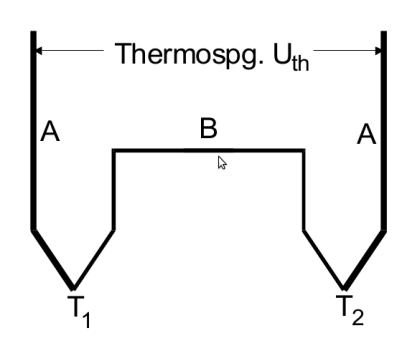
\includegraphics[scale=0.4]{thermo.png}
\caption{Aufbau eines Thermoelements}
\end{figure}
Eine Verbindungstelle befindet als Referenztemperatur sich in einem Gef\"a\ss\ mit Eiswasser. Die Andere wird an der Stelle, an der die Temperatur ermittelt werden soll, angebracht. Mit einem Voltmeter kann nun eine Thermospannung $U_{th}$  gemessen werden. Zwischen $U_{th}$ in mV und der zu messenden Temperatur $T$ in $^\circ C$ ist folgender Zusammenhang gegeben:
\begin{equation}
T = 25.157\cdot U_{th} - 0.19\cdot U_{th}^2.
\end{equation} 



\subsection{Messprogramm}
Die Messung wurde, wie oben beschrieben f\"ur, die Metalle Aluminium und Blei jeweils dreimal durchgef\"uhrt. Dabei wurden die Proben in einem Wasserbad auf eine Temperatur von fast 100$^\circ C$ erhitzt. In das Kalorimeter wurde eine Menge von ca. $600\,m\ell$ eingebracht. Die genaue Masse $m_w$ wurde mit einer Waage bestimmt, mit der auch die Probenmasse $m_k$ bestimmt wurde. Kurz vor dem Einbringen der Probe in das Kalorimeter wurden sowohl die Probentemperatur $T_k$, als auch die Temperatur das Wassers $T_w$ gemessen. Der Temperaturausgleich im Kalorimeter wurde durch einen Magnetr\"uhrer beschleunigt. Hatte das Wasser im Dewargef\"a\ss\ vor dem n\"achsten Versuchsteil eine Temperatur von \"uber 30$^\circ C$, so wurde es gewechselt. Auch die Messung zur Bestimmung der W\"armekapazit\"at der Kalorimeterw\"ande wurde dreimal durchgef\"uhrt. Es wurden jeweils ca. $330\,m\ell$ Wasser erhitzt und mit der gleichen Menge kaltem Wassers gemischt.

\section{Auswertung}
Zunächst wurde die Wärmekapazität $c_gm_g$ des Kalorimeters bestimmt. Dazu wurden folgende Messwerte ermittelt:
\begin{table}[h]
\centering
\begin{tabular}{|c|c|c|}
\hline
 $U_{kalt}[mV]$ &$U_{warm}[mV]$ &$U_{misch}[mV]$\\
\hline
0.85 & 4.10 & 2.06 \\
0.91 & 4.10 & 2.13 \\
0.90 & 4.09 & 2.12 \\
\hline
\end{tabular}
\caption{Spannungen - Messwerte}
\end{table}


\begin{table}[h]
\centering
\begin{tabular}{|c|c|c|c|c|}
\hline
$T_{kalt}[K]$ & $T_{warm}[K]$ & $T_{misch}[K]$ & $m_{kalt}[Kg]$ & $ m_{warm} [Kg]$ \\
\hline
294.40 & 373.10 & 324.17 & (0.37292$\pm$0.00020) & (0.27308$\pm$0.00014)\\
295.89 & 373.10 & 325.87 & (0.37441$\pm$0.00020) & (0.27173$\pm$0.00014)\\
295.64 & 372.86 & 325.63 & (0.37300$\pm$0.00020) & (0.27305$\pm$0.00014)\\
\hline
\end{tabular}
\caption{Wärmekapazität des Kalorimeters - Messwerte}
\end{table}



\section{Diskussion}


\section{Literaturverzeichnis}

\section{Anhang}

\end{document}
